\input{./econtexRoot}\input{\econtexRoot/LaTeX/econtexPaths} 
\documentclass[titlepage]{\econtex} 
\usepackage{xr-hyper}
\usepackage{graphicx}
\usepackage{float}
\graphicspath{ {./Pictures/} }
\input{\econtexRoot/LaTeX/econtexPaths}

\input{\ResourcesDir/owner}

\providecommand{\texname}{OptimlTaxHeight}
\usepackage{\LaTeXFiles/BufferStockTheory}

\begin{document}

\providecommand{\versn}{}
\ifthenelse{\boolean{ifWeb}}{  \renewcommand{\ushort}{\underline}\renewcommand{\versn}{Web} }{} 

\hfill{\tiny \jobname~\versn~\today~{at} \DTMcurrenttime, \input{\ResourcesDir/.git-source-commit}~~\input{\ResourcesDir/.git-public-commit}}

\title{Precautionary Savings, Illiquid Assets, and The Aggregate Consequences of Shocks to Household Income Risk}

\author{Christian Bayer, Ralph Luetticke, Lien Pham-Dao and Volker Tjaden \\ Ballpark by: Sinem Yagmur Toraman\authNum}

\keywords{Incomplete markets, nominal rigidities, uncertainty shocks}

\jelclass{E22, E12, E32\\
  \href{https://econ-ark.org}{\includegraphics{\ResourcesDir/PoweredByEconARK}}
}

\renewcommand{\forcedate}{January,2019}
\date{\forcedate}

\maketitle 
\hypertarget{abstract}{}
\begin{abstract}
  The paper discusses macroeconomic implications of the large income uncertainty faced by the households over the business cycle with a dynamic stochastic general equilibrium model incorporating incomplete markets, liquid and illiquid assets and nominal rigidity.The model produces results matching with the empirical response of portfolio liquidity and aggregate activity to unanticipated changes in the idiosyncratic income uncertainty. Welfare implications of the uncertainty shocks and the policy response are found to be considerably related to the asset position of the households.\\
  The features that differentiates this paper from the previous literature are:\\
 -  The portfolio adjustment as a new channel through which uncertainty affects real activity,\\
 -  The focus on idiosyncratic income risk,\\
 -  Isolation of precautionary savings and portfolio channel of income uncertainty,\\
 -  Introduction of two asset structure,\\
 -  The investigation of distributional consequences of systematic monetary and fiscal policy with an emphasis on potfolios.
\end{abstract}

\begin{authorsinfo}
  \name{Contact: \href{mailto:}{\texttt{storama1@jhu.edu}}, Department of Economics, Wyman Hall, Johns Hopkins University, Baltimore, MD 21218, \url{https://github.com/sytoraman/ballpark/tree/master/models/We-Would-Like-In-Econ-ARK}}
\end{authorsinfo}

\newcommand{\thankstext}{Thank you to Prof. Christopher D. Carroll for the template on which this paper is written.}

\ifthenelse{\boolean{ifWeb}}{}{\thanks{\thankstext}}

\titlepagefinish

\ifthenelse{\boolean{ifWeb}}{\medskip \noindent {\tiny
    \thankstext \medskip \medskip \medskip
  }}{\pagebreak 
}

\ifthenelse{\boolean{ifWeb}}{\medskip \noindent {\footnotesize \thankstext} \\  {\centering \medskip \medskip \medskip  \noindent \hrule height 0.4pt depth 0.0pt width \textwidth \relax}}{\pagebreak } % \end{Web}

\hrule height 0.4pt depth 0.0pt width \textwidth \relax

\medskip \medskip

\hypertarget{Overview}{}
\section{Overview}

 The motivation behind the paper is to investigate the impact of precationary savings motive on the formation of household portfolios when the assets differ with respect to their liquidity and the markets are incomplete.

 \hypertarget{Two Asset Structure}{}
 \subsection{Two Asset Structure}
 
 Households can hold two types of assets for consumption smoothing:\\
 - Liquid (low return) nominal bonds,\\
 - Illiquid (high-dividend-paying) physical capital (modeled by transaction costs)\\
 Two asset structure allows them to differentiate between savings and physical investment. In that way, they can produce a much stronger response in aggregate demand to income risk compared to the standard Aiyagari (1994) model, where physical capital is the only source for savings.

\hypertarget{Incomplete Markets}{}
\subsection{Incomplete Markets}

 In order to produce aggregate output effects from the fluctuations in demand, they introduce sticky prices a la Rotemberg (1982)

\hypertarget{Two Types of Households}{}
\subsection{Two Types of Households}

  Introduction of two different types of households, namely, workers and entrepreneurs, is helpful in the following aspects:\\
- It enables the allocation of pure rents without distorting factor returns and without introducing another tradable asset,\\
- Wealth distribution is better matched as it allows a transitory state in which incomes are extremely high.
 
\hypertarget{Estimation of Income Risk Over Time}{}
\section{Estimation of Income Risk Over Time}

First, authors report their procedure for estimation of the household income and its shock. They follow the framework outlined by Storesletten, Telmer, and Yaron (2001, 2004), but without restricting themselves to a general business cycle relationship. For that purpose, they collected  the data from Survey of Income and Program Participants (SIPP) for the period between 1984-2013.

\hypertarget{Income Process}{}
\subsection{Income Process}

Their data is restricted to housholds between the age of 30-56 and the labor income of the household is given by:\\
\begin{align}
logy_{it} = f(o_{it}) + \tau_{it} + h_{it} + \mu_{i}\\
     h_{it} = \sum_{s=c}^{t}\rho_{h}^{t-s}\varepsilon_{is}^{h}\\
    \tau_{it} = \varepsilon_{it}^{\tau} + \rho_{\tau}\varepsilon_{it-1}^{\tau} \\
     \varepsilon_{it}^{\tau} \thicksim \mathcal{N}(0,\sigma_{\tau}^{2}),   \varepsilon_{it}^{h} \thicksim \mathcal{N}(0,\sigma_{\varepsilon,t}^{2}),   \mu_{i}\thicksim \mathcal{N}(0,\sigma_{\mu}^{2})
\end{align}
where c is the cohort by the quarter when the head of the household turns 30, $f(o_{it})$ measures  the observable characteristics$ o_{it}$, $ \tau_{it}$ is MA(1) transitory shock, $ \mu_{i}$ is the fixed effect and $h_{it}$ is the persistent component.

\hypertarget{Risk Process}{}
\subsection{Risk Process}

Transitory shocks and fixed effects are assumed to be homoscedastic. Variance of the shocks $\varepsilon_{it}^{h}$ to the persistent component follows an AR(1) process:\\
\begin{align}
    \sigma_{\varepsilon,t}^{2} = \bar{\sigma_{\varepsilon,t}^{2}}exp(s_{t}+t\theta_{1}+t^{2}\theta_{2})\\
    s_{t+1} =\rho_{s}s_{t}+ \varepsilon_{t}^{s}\\
  \varepsilon_{t}^{s} \thicksim \mathcal{N}\left(-\dfrac{\sigma_{s}^{2}}{2(1+\rho_{s})},\sigma_{s}^{2}\right)\\
  \end{align}
  For the estimator, their methodology is an extension of the method of moments estimator for the income risk by Storesletten, Telmer, and Yaron (2001, 2004). However, the authors provide a reformulation in terms of a quasi-maximum-likelihood estimator. The parameter estimates are given in Table 1.

  \begin{table}[H]
  \centering
    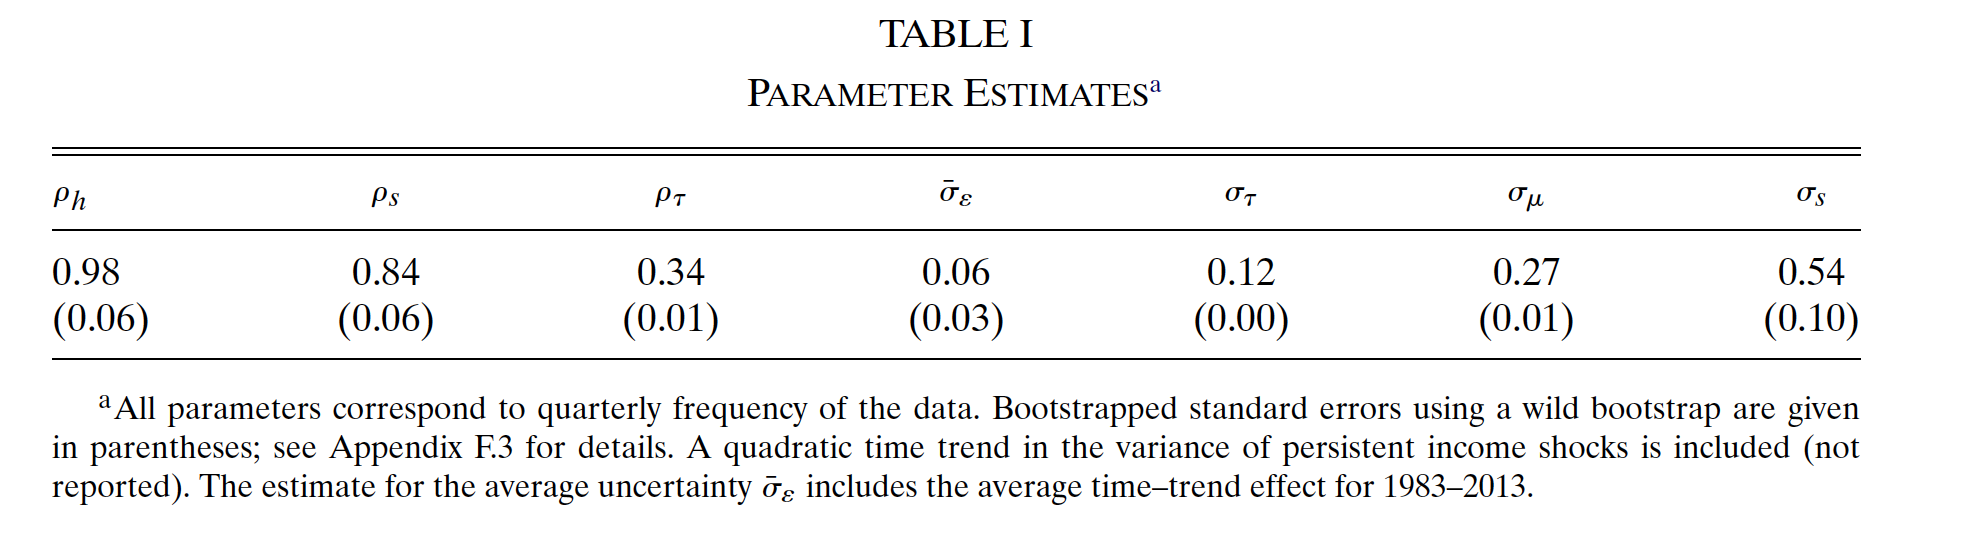
\includegraphics[width=0.8\textwidth]{Table1.png}
  \end{table}

\hypertarget{Responses to Shocks to Income Risk}{}
\section{Responses to Shocks to Income Risk}
  
\hypertarget{Aggregate Response}{}
\subsection{Aggregate Response}

They report that increase in income risk induces a decrease in aggregate output, investment and an increase in the return premium of illiquid assets which can be seen below in Figure 3.\\
Furthermore, they highlight the strong reaction of the investment, compared to the aggregate output, and its repercussions on the balance sheet of households. An increase in the income risk is found to result in an increase in the ratio of liquid to illiquid assets. They provide a rationale for the increase in portfolio liquidity by analyzing the movements in housing prices and liquidity premium, where the movements in the latter being the main contributor.

\begin{figure}[H]
  \centering
  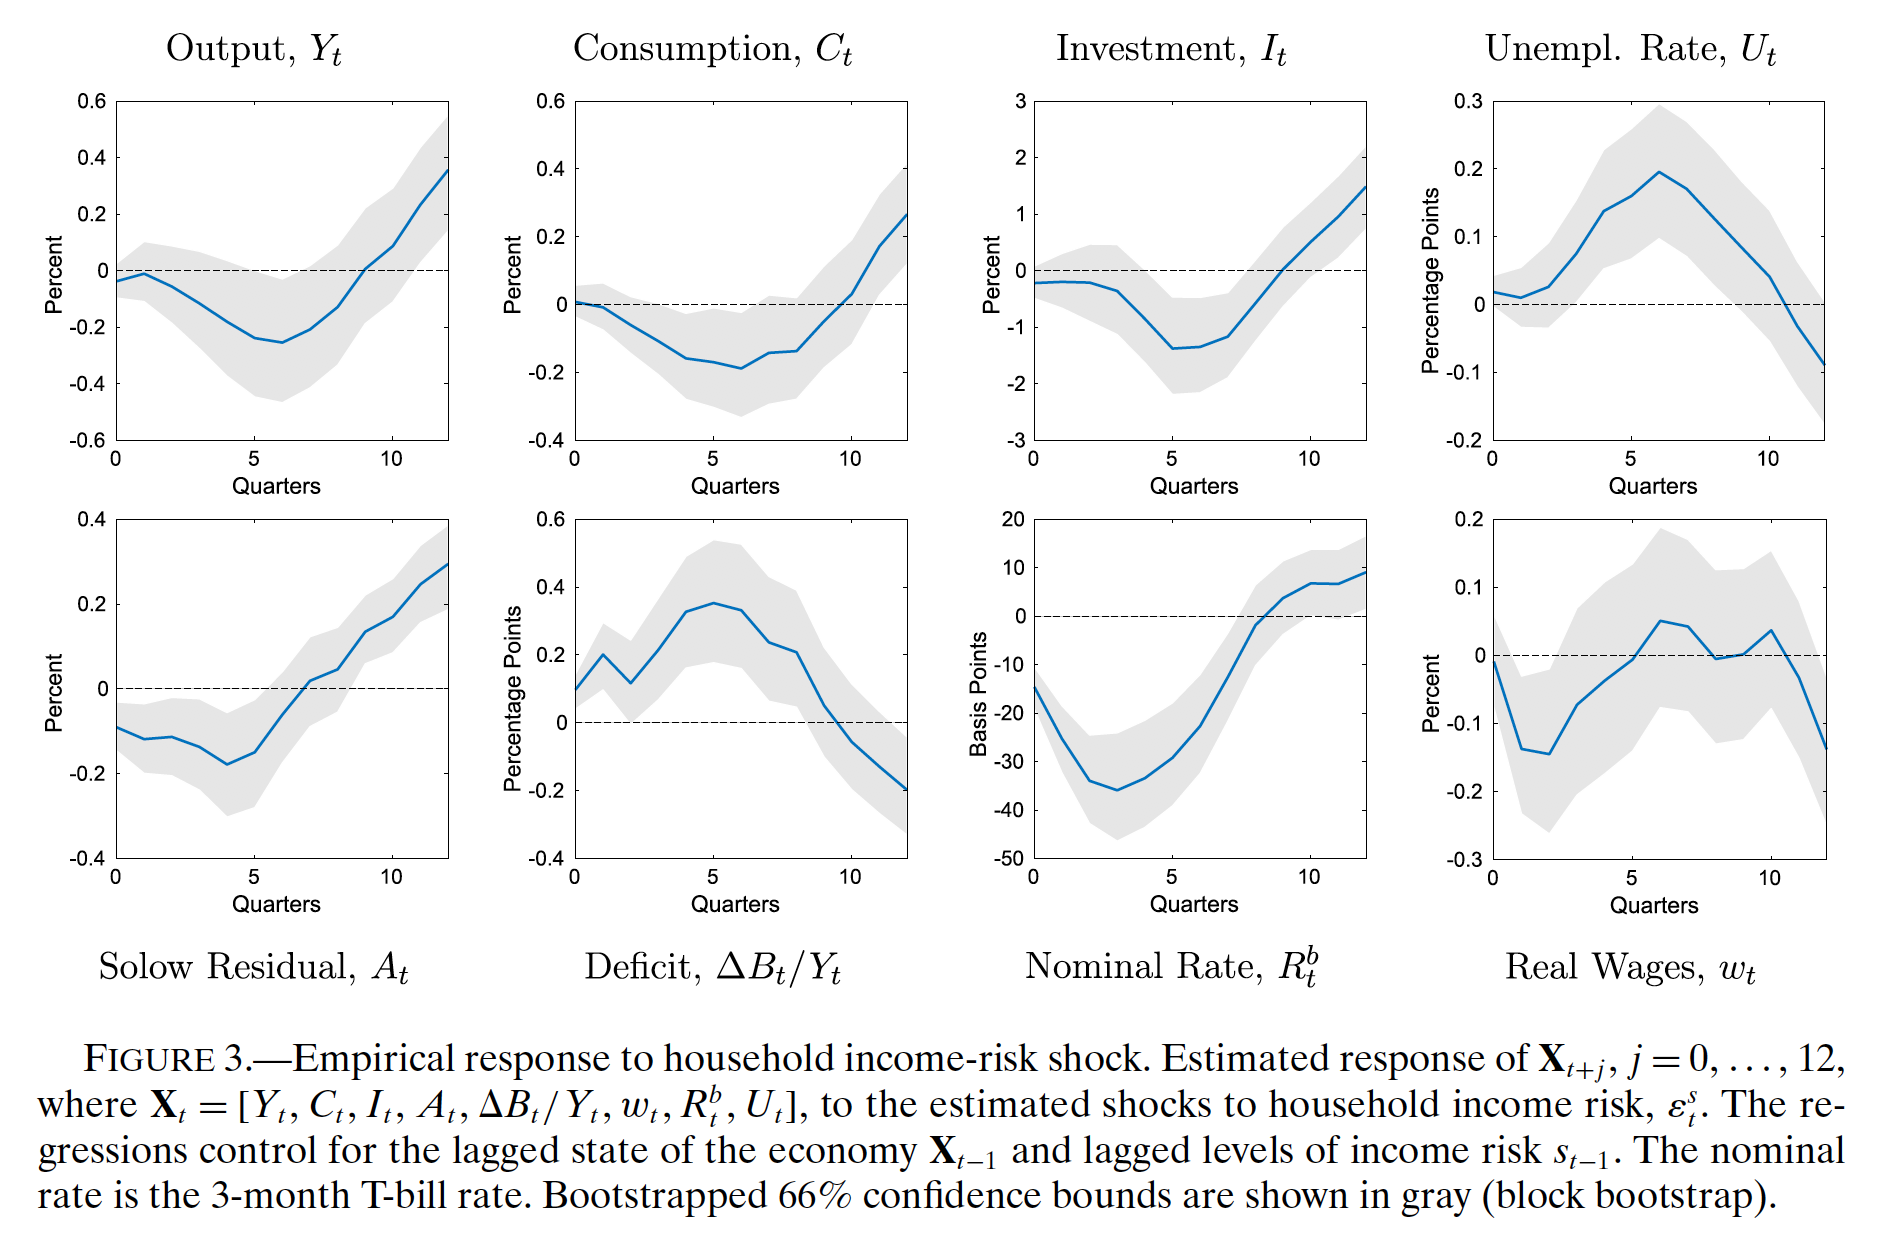
\includegraphics[width=1\textwidth, height=12cm]{Figure3.png}
  \end{figure}

\hypertarget{Response by Wealth Group}{}
\subsection{Response by Wealth Group}

They analyze the impact of income risk by taking into account the heterogeneity among households. The analysis relies on the data collected for 1983-2013 from Survey of Consumer Finances (SCF) focusing on households, whose head is the age of 30-55 and with at least two adults and married.\\
Figure 5 reports the results, showing that the increase in liquidity holdings is much stronger when the household is relatively poorer.

\begin{figure}[H]
  \centering
  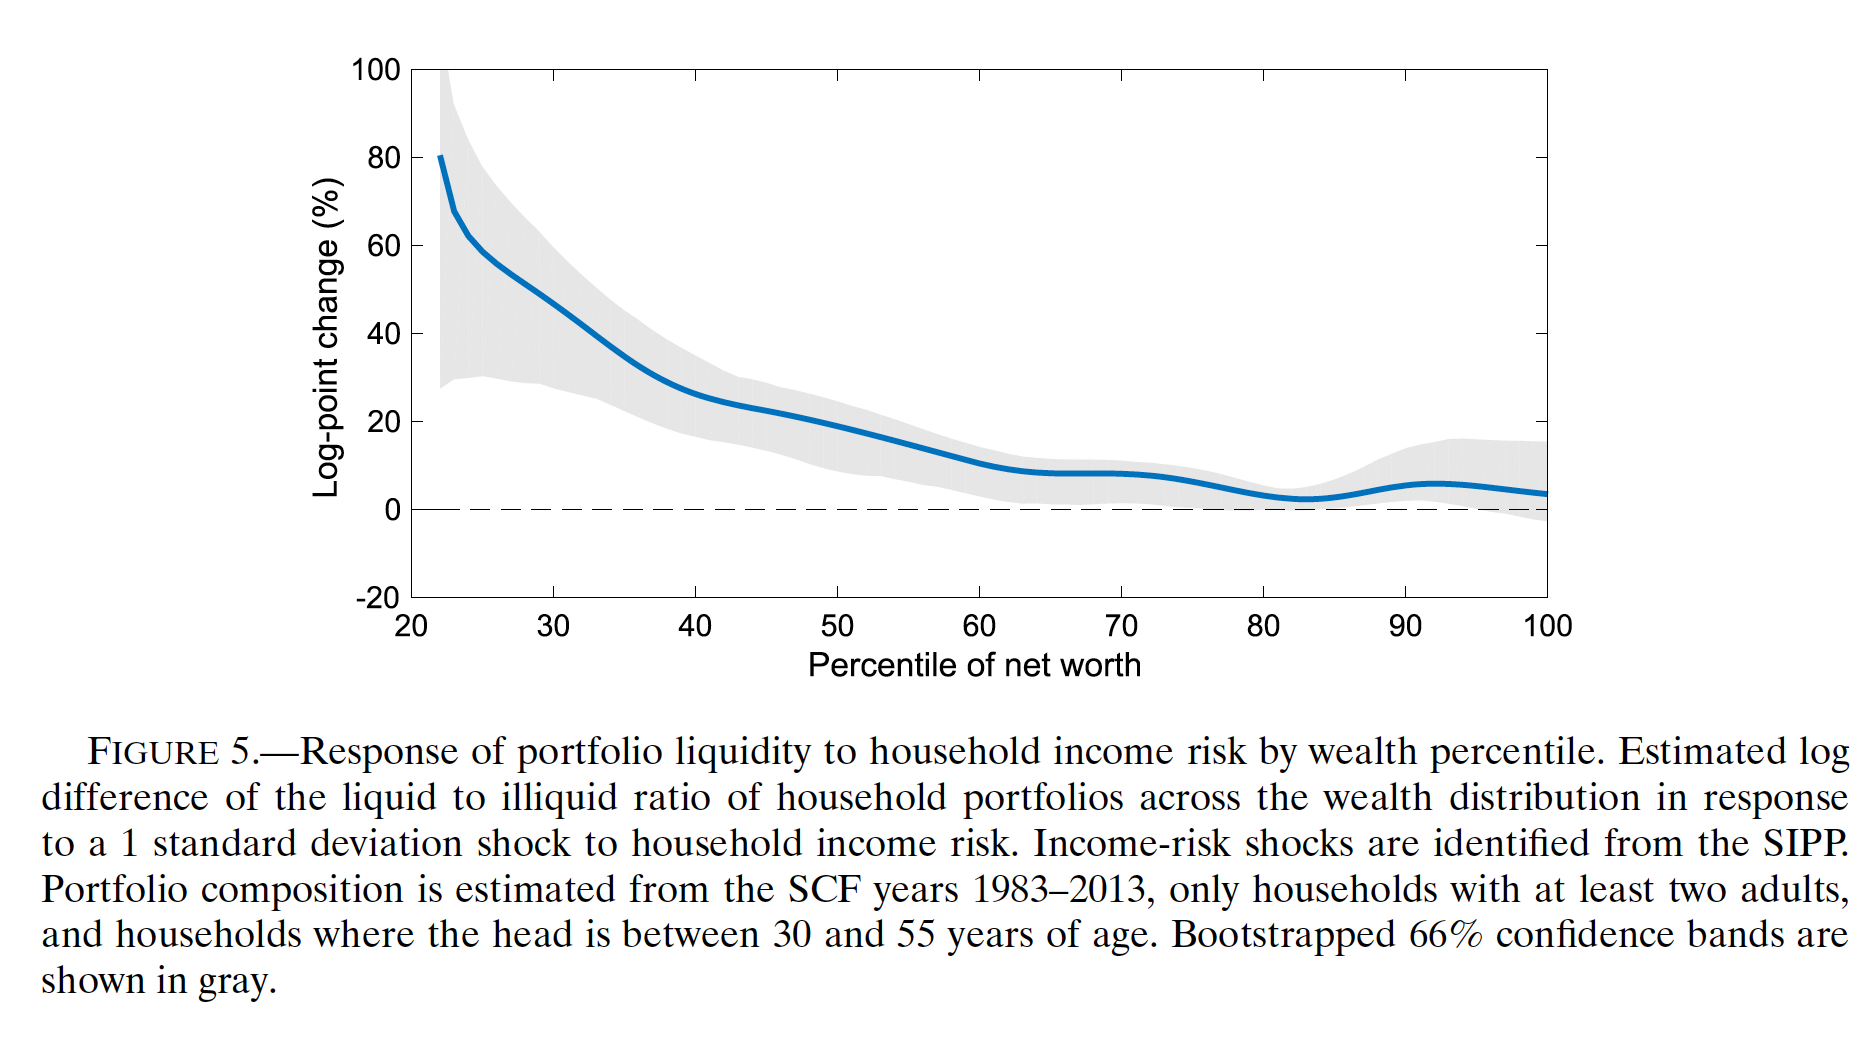
\includegraphics[width=1\textwidth, height=12cm]{Figure5.png}
  \end{figure}

\hypertarget{The Model}{}
\section{The Model}

The authors provide a simple partial equilibrium model and a quantitative general equilibrium model. Here, I will only report the quantitative one:\\
It is a dynamic heterogenous households model with\\
- incomplete markets,\\
- time variations in income risks and\\
- sticky prices (a la Rotemberg (1982)).
\hypertarget{Agents}{}
\subsection{Agents}

\hypertarget{Households}{}
\subsubsection{Households}

- Unit mass of ex ante identical, infinitely lived households\\
- Time separable preferences described by Greenwood$-$Hercowitz$-$Huffman (GHH) preferences\\
- Derive felicity from consumption, $c_{it}$, and leisure\\
- Earn income from supplying labor $n_{it}$, renting out capital $k_{it}$, interest on bonds $b_{it}$\\
- Holdings of capital is adjusted by incurring a felicity cost, $\chi_{it}$, which is i.i.d. from a logistic distribution\\
- Holdings of bonds are above $ \underline{B} $, and holdings of capital are nonnegative\\
- Nonparticipants of the capital market still get dividends and able to adjust bond holdings\\
- There is a wasted intermediation cost of $\bar{R}$
The sector for households consists of workers and entrepreneurs, where the transition between two states is stochastic. They both rent out physical capital and have the ability to self-insure themselves against the income-risk through saving in bonds (liquid nominal asset) and capital (less liquid physical asset). However, the two types of households differ in the sense that only workers supply labor and entrepreneurs do not work, but earn pure rents.\\
- Productivity evolves randomly. given by
-  Variance of the shocks to productivity is given by the following set of equations:\\
\begin{align}
    \sigma_{h,t}^{2}={\bar{\sigma}}_{h}^{2}exps_{t}\\  
    s_{t+1} =\rho_{s}s_{t} + \varepsilon_{t}^{s}\\    
    \varepsilon_{t}^{s} \thicksim \mathcal{N}\left(-\dfrac{\sigma_{s}^{2}}{2(1+\rho_{s})},\sigma_{s}^{2}\right)
\end{align}
- Households maximize the discounted sum of felicity:\\
\begin{align}
   E_{0} = max _{{c_{it},n_{it},\Delta k_{it}}} \sum_{t=0}^{\infty} \beta^{t} u[cn-G(h_{it},n_{it})]-\mathbb{1}_{\Delta_{k_{it}\neq0}} \chi_{it} 
\end{align}
subject to the budget constraint:\\
\begin{align}
c_{it}+b_{it}+q_{t}k_{it+1} =b_{it}\dfrac{R(b_{it},R_{t}^{b}}{\pi_t} +(q_{t}+r_{t})k_{it}+(1-\tau)(w_{t}h_{it}N_{t} + \mathbb{1}_{h_{it}=0} \Pi_{t}),\\
k_{it}\geq 0,\\
b_{it+1}\geq \underline{B}
\end{align}
where $\chi_{it}$ is the utility cost of adjustment and  $x_{it}= c_{it}-G(h_{it},n_{it})$.
G measures the disutility from work and
\begin{align}
  c_{it} = \left(\int c_{ijt}^{\dfrac{\eta-1}{\eta}}dj\right)^{\dfrac{\eta}{\eta-1}}
\end{align}
Moreover,$b_{it}$ is the real bond holdings, $\underline{B}$ is the exogenous borrowing constraint, $k_it$ is the amount of illiquid asset, $q_{t}$ is the price of illiquid asset,  $r_t$ is dividend, $\pi_{t}=\dfrac{P_t}{P_{t-1}}$ is realized inflation,  $R$ is nominal gross return on bonds, $R_t^b$ is the Central Bank's interest rate.\\
- Felicity function u exhibits CRRA with $\xi$>0 denoting the risk aversion parameter:\\
\begin{align}
  u(x_{it})=\dfrac{1}{1-\xi}x_{it}^{1-\xi}
\end{align}
- There are 3 functions characterizing the problem of the household:\\
\begin{align}
V_{a}(b,k,h:\Theta,R^{b},s) = max_{k',b'_{a}}u[x(b,b'_{a},k,k',h)]+\beta EV(b'_{a},k',h',\Theta',R^{b'},s')\\
V_{n}(b,k,h:\Theta,R^{b},s) = max_{k',b'_{n}}u[x(b,b'_{n},k,k',h)]+\beta EV(b'_{n},k',h',\Theta',R^{b'},s')\\
EV(b',k',h:\Theta,R^{b},s) = E_{\xi',h',s'} {max[V_{a}(b',k',h';\Theta',R^{b'},s') - \xi', V_{n}(b',k',h';\Theta',R^{b'},s')]}
\end{align}

\hypertarget{Intermediate-Goods Producers}{}
\subsubsection{Intermediate-Goods Producers}

- CRS production function\\
\begin{align}
  Y_{t} = N_{t}^{\alpha}K_{T}^{1-\alpha}
\end{align}
- They maximize profit\\
\begin{align}
MC_{t}Y_{t} -w_{t}N_{t} -(r_{t}\delta)K_{t} = MC_{t}N_{t}^{\alpha}K_{T}^{1-\alpha} - w_{t}N_{t}-(r_{t}+\delta)K_{t}
\end{align}
- Perfectly competitive markets\\
\begin{align}
  w_t = \alpha MC_{t}\left(K_{t}/N_{t}\right)^ {1-\alpha}, r_{t}+\delta = (1-\alpha)MC_{t}(N_{t}/K_{t})^{\alpha}
\end{align}

\hypertarget{Final-Goods Producers}{}
\subsubsection{Final-Goods Producers}

- Price adjustment costs by Rotemberg (1982)\\
- Risk neutral managers compensated by a share in profits\\
- Not participating in the asset market\\
- With quadratic costs of adjustment they maximize\\
\begin{align}
   E_{0} \sum_{t=0}^{\infty} \beta^{t} Y_{T} \left \lbrace \left(\dfrac{p_{jt}}{P_{t}}-MC_{t}\right)\left(\dfrac{p_{jt}}{P_{t}}\right )^{-\eta} - \dfrac{\eta}{2 \kappa} \left (log\dfrac{p_{jt}}{p_{jt-1}} \right)^{2} \right \rbrace 
  \end{align}
  - Phillips curve is given by\\
  \begin{align}
    log(\pi_{t})=\beta E_{t}\left [log\left(\pi_{t+1}\right)\dfrac{Y_{t+1}}{Y_{t}}\right]+ \kappa\left (MC_{t} - \dfrac{\eta-1}{\eta} \right)
   \end{align}
  
\hypertarget{Government}{}
\subsubsection{Government}

- Monetary authority: Nominal interest rates on liquid assets  are set according to\\
\begin{align}
  \dfrac{R_{t+1}^{b}}{\bar{R}^{b}} =\left( \dfrac{R_{t}^{b}}{\bar{R}^{b}}\right)^{2}\left(\dfrac{\pi_{t}}{\bar{\pi}}\right)^{(1-\rho R)\theta_{t}}
  \end{align}  
  - Fiscal authority: Issuance of government bonds according to\\
  \begin{align}
\dfrac{B_{t+1}}{\bar{B}}= \left( \dfrac{B_{t}R_{t}^{b}/ \pi_{t}}{\bar{B}\bar{R}^{b}/ \bar{\pi}}\right)^{\rho B} \left(\dfrac{\pi_{t}}{\bar{\pi}} \right)^{-\gamma \pi} \left( \dfrac{\mathcal{T}}{\bar{\mathcal{T}}} \right)^{-\gamma \mathcal{T}}
\end{align}

\hypertarget{Numerical Implementation}{}
\section{Numerical Implementation}

The dynamic program is not computable as it involves the infinite-dimensional object $\Theta_{t}$. Thus, the distribution of $\Theta_{t}$ is discretized by a histogram.\\
Household's planning problem is solved by the application of an endogenous grid-point method originally developed by Carroll (2006). The idiosyncratic productivity process is approximated by a discrete Markov chain consisting of 26 states.\\

\hypertarget{Results}{}
\section{Results}

The results are based on the parameters that are calibrated to match the characteristics of the U.S. economy for the period between 1983-2015. Here, I will provide a summary of their results.

\hypertarget{Household Portfolios and The Individual Response to Income Risk}{}
\subsection{Household Portfolios and The Individual Response to Income Risk}

First, the response of individual households is reported in a partial equilibrium setting which can be seen from Figure 7. It has been reported that:\\
- Consumption declines for all households\\
- Increase in income risk makes households consume less and save more in liquid form by selling illiquid capital\\
- Portfolio liquidity increases for all households\\
Second, the authors report the results for the general equilibrium setting, where prices are allowed the adjust and the expectations are consistent with the competitive equilibrium (Figure 8):\\
- Poor households use liquidity for consumption smoothing as a consequence of the fall in wage incomes\\
- Rich entrepreneur households experience a temporary increase in income as the pure profits increase in equilibrium, and thus, invest in liquid assets\\
- Lower middle class exhibits the strongest increase in the portfolio liquidity

\begin{figure}[H]
  \centering
  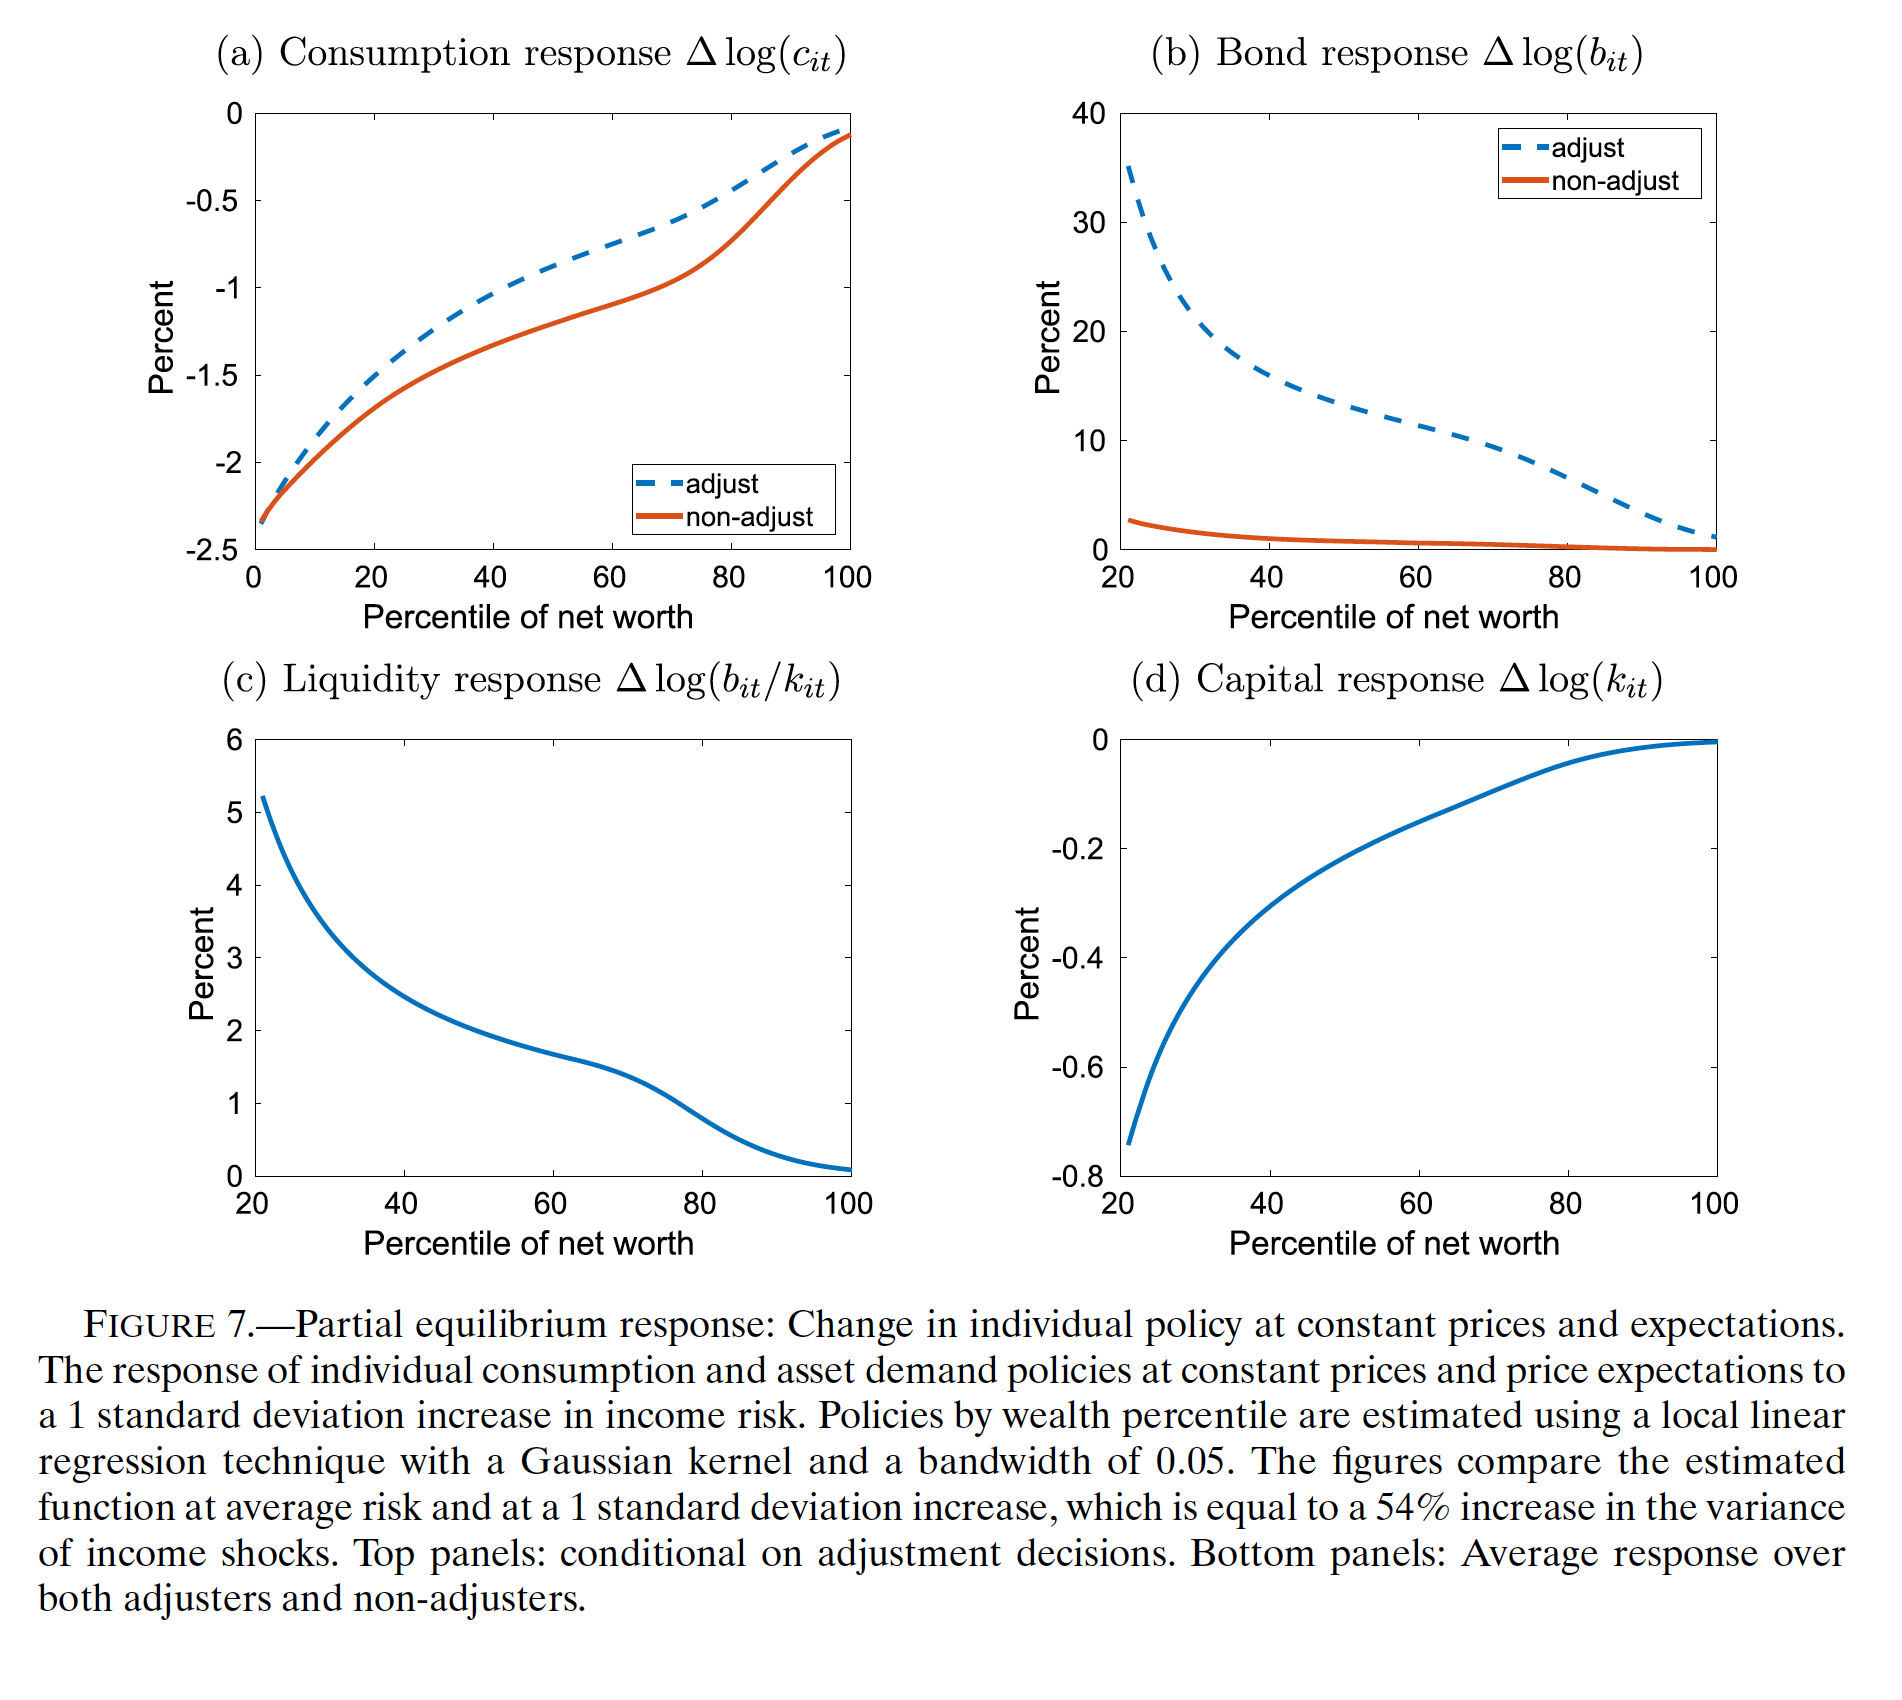
\includegraphics[width=1\textwidth, height=12cm]{Figure7.png}
  \end{figure}

  \begin{figure}[H]
  \centering
  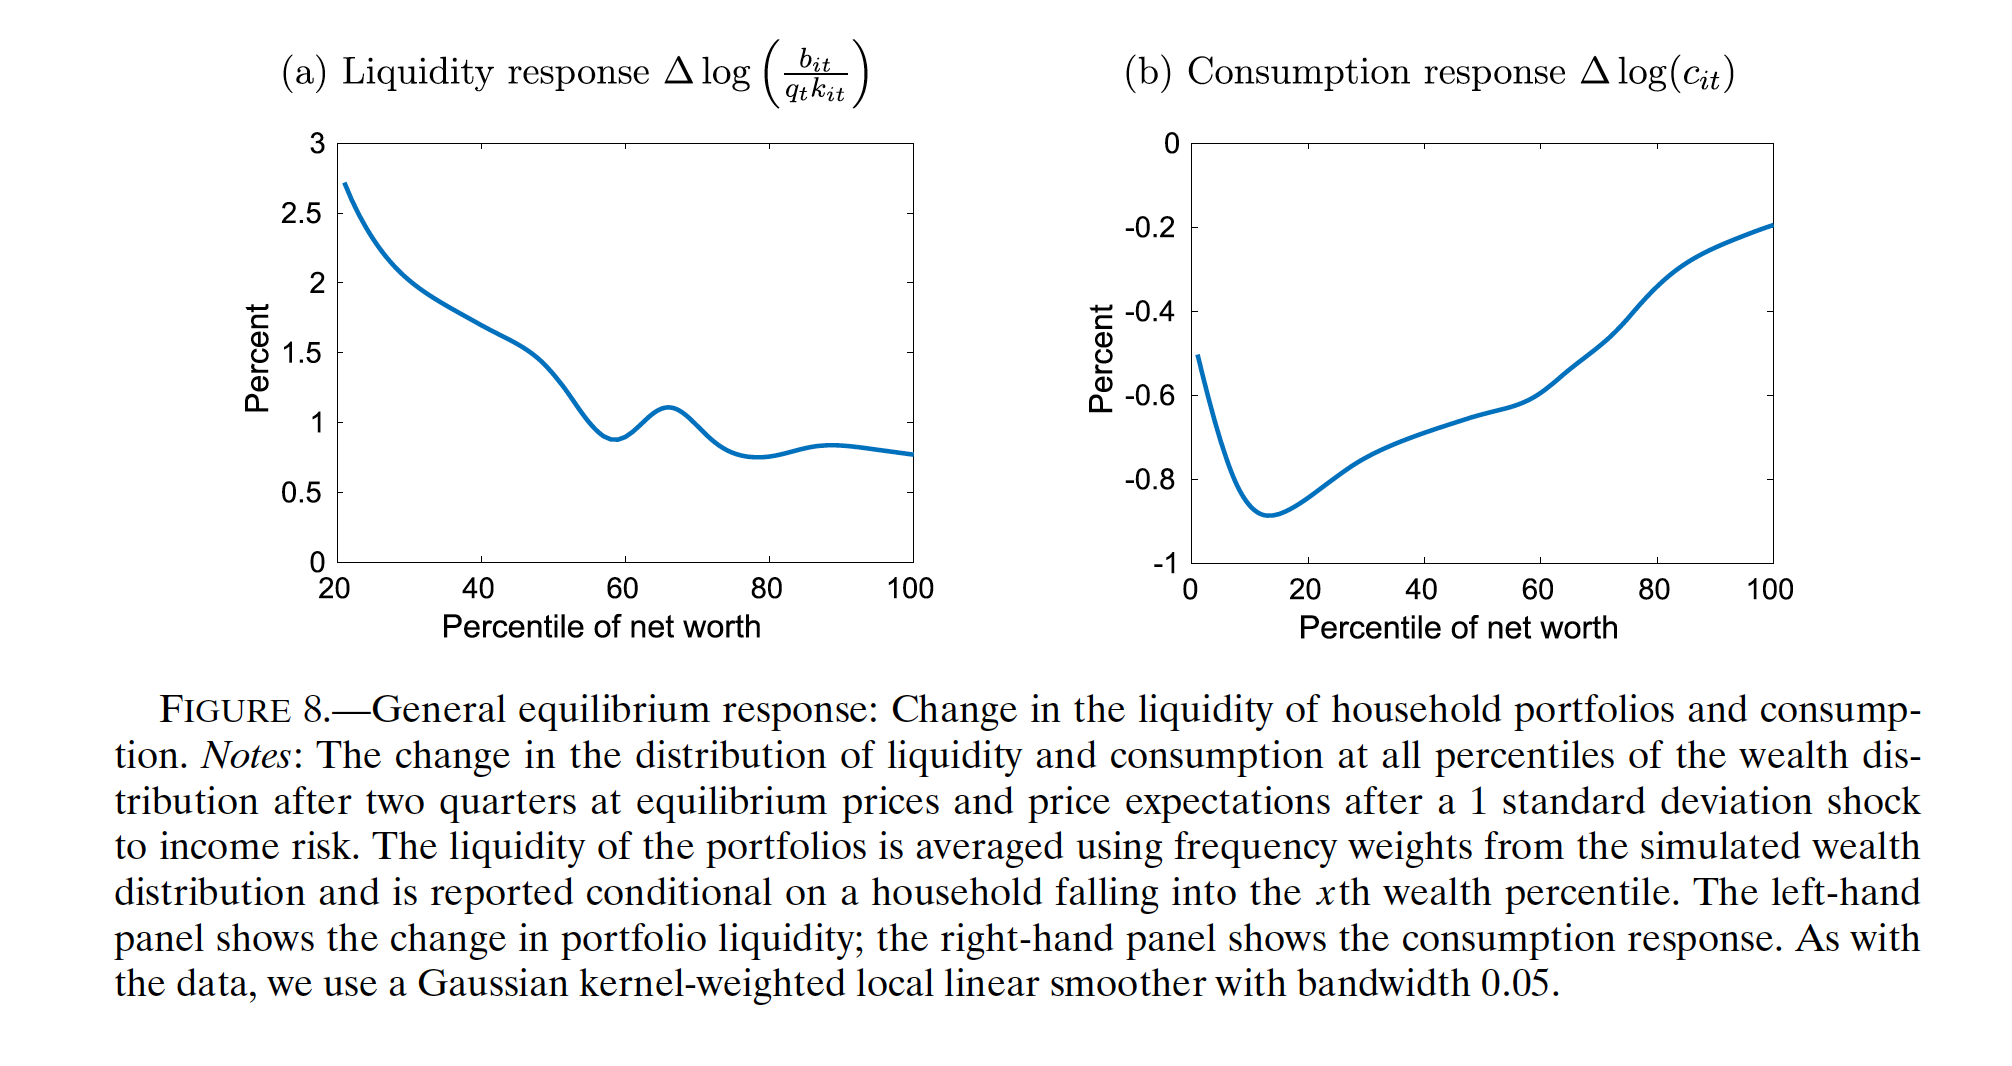
\includegraphics[width=1\textwidth, height=12cm]{Figure8.png}
  \end{figure}

\hypertarget{Aggregate Consequences of Shocks to Household Income Risk}{}
\subsection{Aggregate Consequences of Shocks to Household Income Risk}

As a result of an increase in the variance of the income shock by a magnitude of 1 standard deviation:\\
- Output drops by 0.2 percent, recovering only after 12 quarters\\
- Drop in consumption is much larger, recovering only after 20 quarters\\
- Investment experiences the sharpest decline, which is five times larger than that of output\\
- Fluctuations in household income risk captures the 21 percent of the fluctuations in the business cycle\\
They explain the drop in output by the increase in precautionary savings, which goes along with the efforts of households to rebalance their portfolios in favor of the liquid asset. This is motivated by the fact that when the uncertainty is higher, illiquid assets are deemed to be less favorable for consumption smoothing than the liquid assets. Therefore, a drop in both consumption and investment is observed.

\hypertarget{Stabilization Policy}{}
\subsection{Stabilization Policy}

In addition to the baseline calibration of fiscal and monetary policy, they consider two additional scenarios:\\
- perfect stabilization through monetary policy\\
- perfect stabilization through fiscal policy\\
The results can be seen in Figure 10. Decline in consumption is still observed due to the precautionary savings motive.

\begin{figure}[H]
  \centering
  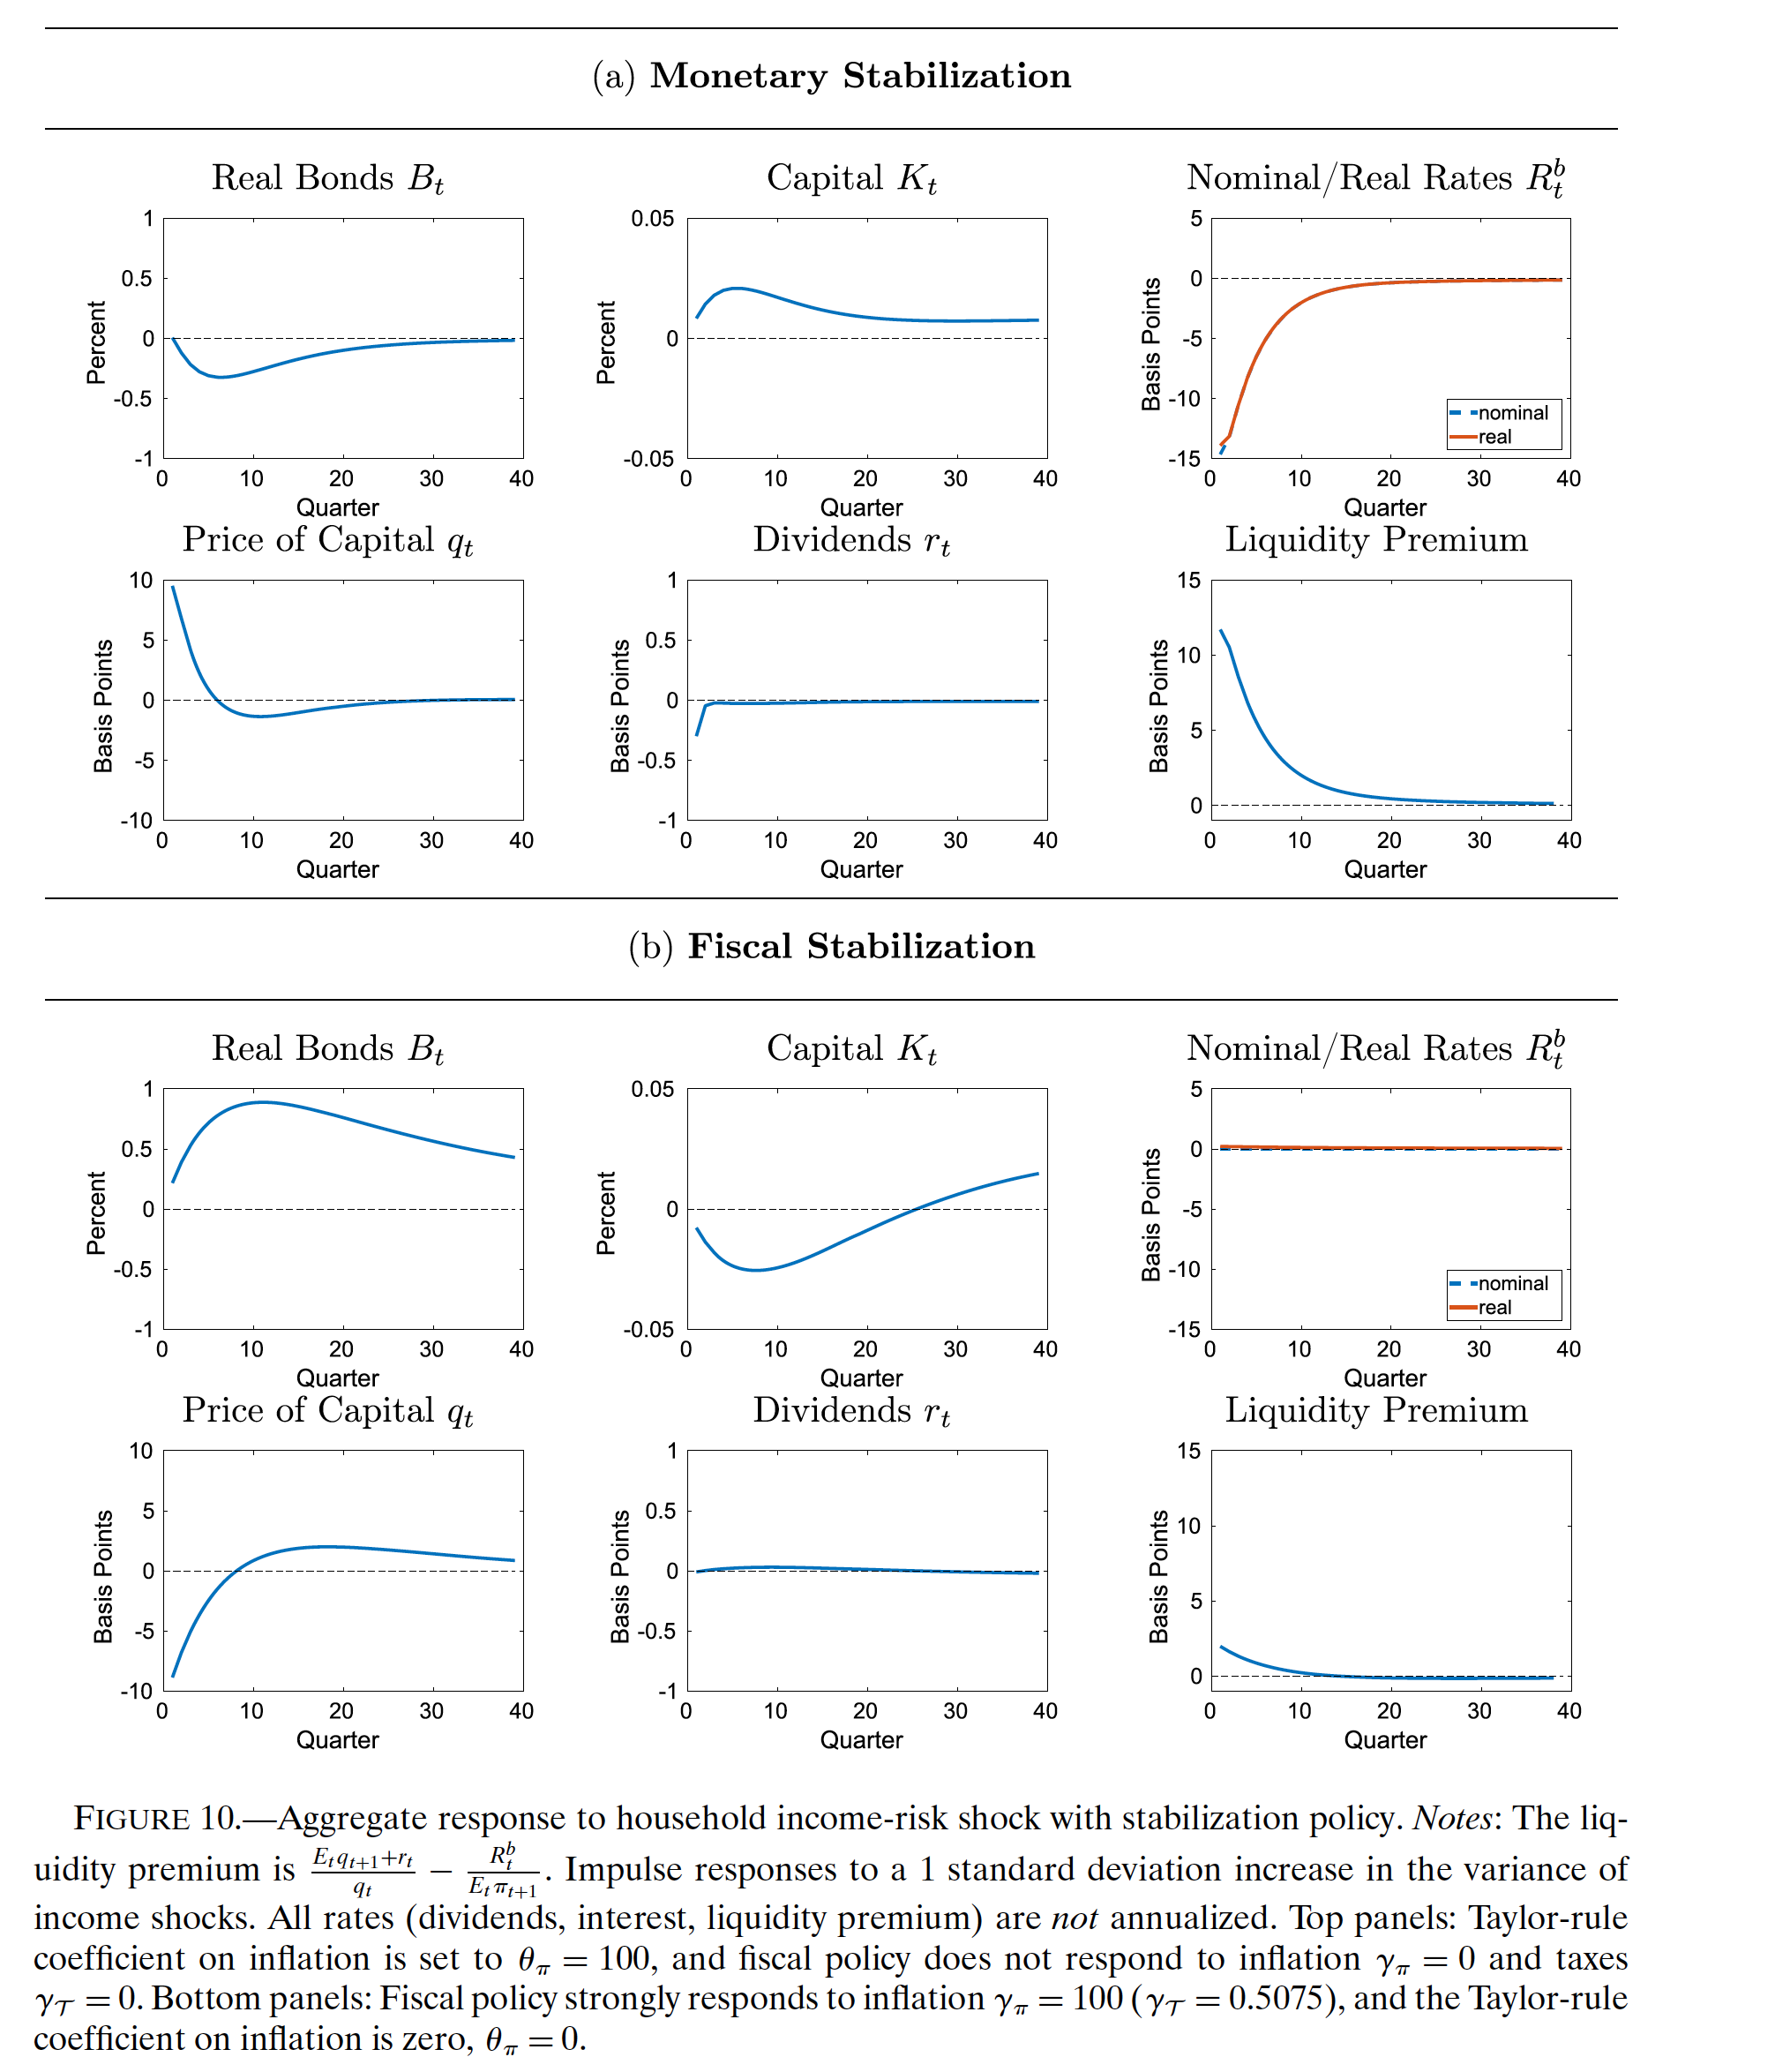
\includegraphics[width=1\textwidth, height=12cm]{Figure10.png}
  \end{figure}

\hypertarget{Redistributive and Welfare Effects}{}
\subsection{Redistributive and Welfare Effects}

An increase in the household income risk worth of 1 percent  standard deviation leads to a decrease in lifetime consumption of 27 basis points on average. However, welfare loss is bigger for households with fewer asset holdings and this result holds for all policy regimes. On the other hand, distributional consequences differ between different stabilization policies:\\
- Fiscal policy benefits people with a higher amount of illiquid wealth\\
- Monetary policy benefits people with a very low levels of wealth, taking from the people with liquid portfolios\\
- For well insured and wealthy households, changes in equilibrium prices are of great importance. Thus, they suffer more from stabilizing monetary policy due to its impact on decreasing asset returns. In contrast, they are better off by a fiscal policy stabilization due to its impact on crowding out the investment and keeping the returns high.

\hypertarget{Conclusions}{}
\section{Conclusions}

By taking into account the price stickiness and incomplete markets along with a framework where households are allowed to allocate their savings between two types of assets, i.e. liquid and illiquid, the paper provides an analysis on the impact of fluctuations in the riskiness of household income through the lens of precautionary savings.  They show that an increase in the income risk induces flight to liquidity as people prefer liquid assets over the illiquid assets for consumption smoothing puposes in the short-run. Therefore, investment along with the consumption also decreases.\\
Compared to the previous literature regarding uncertainty, they introduce the portfolio rebalancing channel to describe how uncertainty can induce a recession. The findings are also helpful in understanding the severity of the Great Recession. Specifically, when 1 standard deviation increase in household income risk is considered, the following results are reported:\\
- Drop in aggregate activity by 0.2 percent  and investment by 1 percent over the first year after the shock,\\
- At ZLB, when neither monetary nor fiscal policy are ineffective in stabilizing the economy, there is a loss of almost 2 percent.\\
Going further, they also show that the results are sensitive to the policy stance and asset position of the household. Accordingly, they emphasize the significance of the supply of liquid funds in the economy.
  
\clearpage\vfill\eject

\onlyinsubfile{\bibliography{\econtexRoot/LaTeX/BufferStockTheory,economics}}

\end{document}

